\begin{figure*}[!t]
\centering
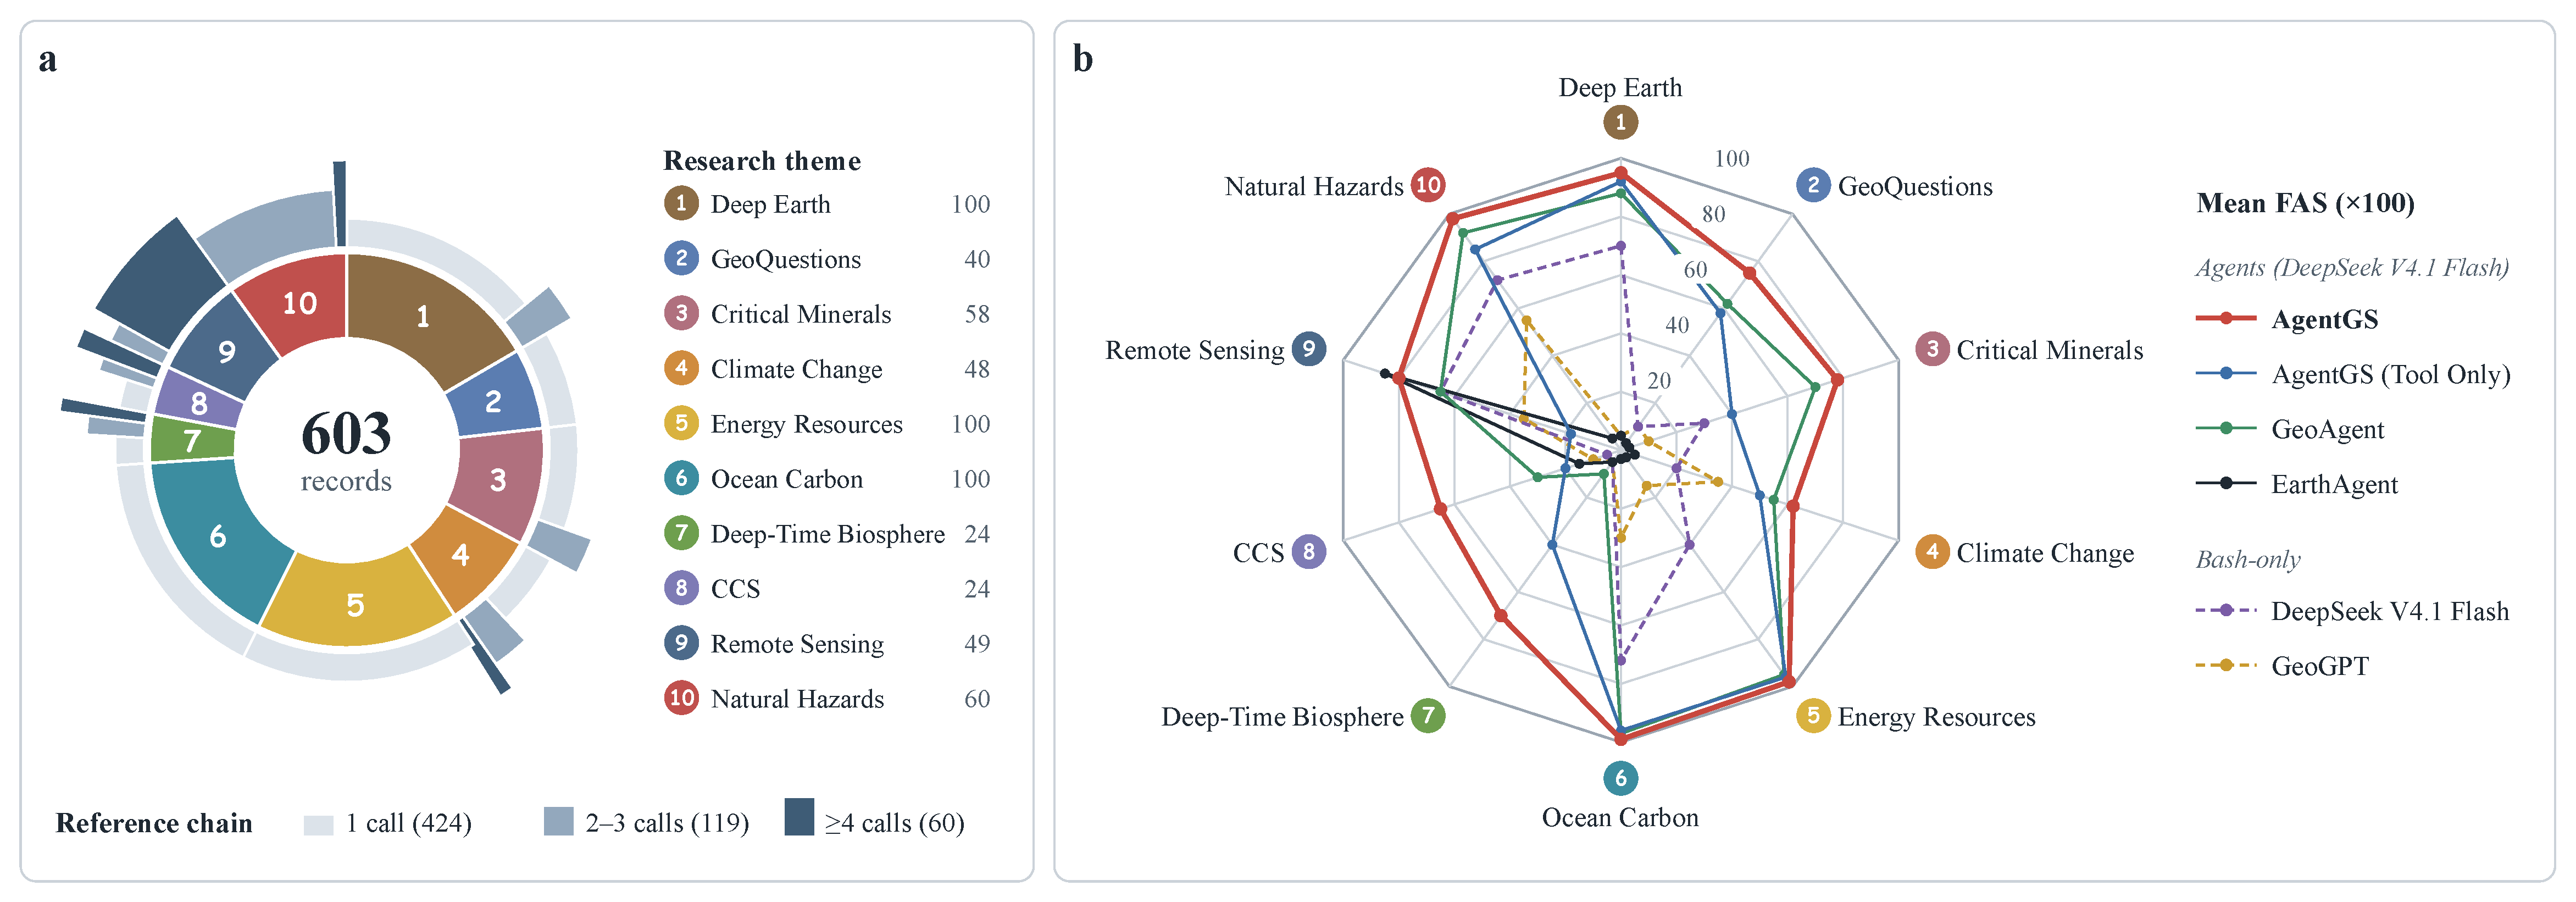
\includegraphics[width=\textwidth]{fig_geotooleval.pdf}
\caption{GeoToolEval composition and domain-specific performance. (a) The 603 evaluation records by research theme (inner ring); outer teeth split each theme by reference-chain length, with longer teeth for longer chains. (b) Mean FAS on each theme. The agent frameworks AgentGS, AgentGS (Tool Only), GeoAgent, and EarthAgent are all evaluated with DeepSeek V4.1 Flash (solid); DeepSeek V4.1 Flash and GeoGPT run as Bash-only agents (dashed).}
\label{fig:geotooleval}
\Description{Panel a is a donut chart: the inner ring divides 603 records among ten numbered research themes, and teeth around it split each theme into records with one, two to three, or at least four reference calls, longer teeth marking longer chains. Panel b is a radar chart over the same ten numbered themes comparing mean FAS of AgentGS, AgentGS with tools only, GeoAgent, and EarthAgent, all using DeepSeek V4.1 Flash, with DeepSeek V4.1 Flash and GeoGPT as Bash-only agents.}
\end{figure*}
